\documentclass[12pt]{article}

\title{The Anti-Global Warming Swindle}
\author{Maximillien Courchesne-Mackie (6168005) \\
             Patrick White (5936927)}
\date{\today}

\usepackage[left=2cm,right=2cm]{geometry}
\usepackage{graphicx}
\graphicspath{{./img/}}
\DeclareGraphicsExtensions{.pdf,.png,.jpg}
\setlength{\parindent}{0in}

\begin{document}
\maketitle
\newpage

\begin{abstract}
    Because global warming is a multi-national phenomenon which directly effect humans, the analysis of scientific evidence is vital. \textit{The Great Global Warming Swindle} is a documentary which masquerades as a scientific commentary on the state of global warming, but fails to provide credible or correct evidence to support it's claims. This report will identify and criticise the arguments fundamental to the view of the director using current peer-reviewed scientific knowledge and common sense.
\end{abstract}
\newpage

\tableofcontents
\newpage

\listoffigures
\listoftables
\newpage

\section*{Summary}
\newpage

\section{Introduction}
	Due to advances in various scientific fields concluding that there has been a significant rise in the Earth's temperature over the past century, the subject of global warming has become a household topic. Politicians have adopted the phenomenon as a major part of their campaign and some parties have made it the root of their platform. \\
	
	This unifying fact has given rise to groups of skeptics who reject the scientific consensus on climate change and put forth the idea that it is a political and economical campaign of fraud. Martin Durkin, the director of \textit{The Great Global Warming Swindle} is one of these skeptics. His film accuses the International Panel on Climate Change (IPCC) of being too political, asserts that man-made $CO_2$ is insignificant as a greenhouse gas and that the developed world is killing the African dream of sustainable development. \\
	
	This report will outline the major arguments Durkin proposes and will show how each of those arguments are either based on false data or poor interpretations of data. Our arguments will be representative of the current scientific consensus on the matter and will be complimented with proven and peer-reviewed data amassed through years of scientific study and analysis. The information will be conveyed in an accessible manner, allowing scientific lay-persons to follow our criticism of the documentary. \\

\section{Global Warming - An Overview}
	\textit{Global warming} is the increase of the temperature of Earth's climate and is usually studied over vast periods of time. The Earth's atmosphere retains a large portion of the heat emitted by the Sun thanks to a group of compounds known as \textit{greenhouse gases}. \textit{Human-caused global warming} is the increase of Carbon Dioxide ($CO_2$) in the atmosphere due to man-made systems which pollute the environment (non-electrical vehicles, mining, and factories for example). \\
	
	To fully understand the impact humans have on the global temperature, we need to understand the greenhouse effect. The greenhouse effect is what allows the Earth to remain heated by the Sun's rays and, without it, Earth would be inhabitable. It is due to a select number of compounds which are able to absorb and emit infrared radiation, called greenhouse gases. These gases form a protective shell around the Earth and absorb the Sun's radiation [...]. \\
	
\section{Arguments Presented}
    \textit{The Great Global Warming Swindle} does not provide any credible evidence to support their claims of a political and economic climate scandal, however the following section will extract the film's arguments and provide rebuttals that are founded in scientific fact.
    
\subsection{The Relevance of the Post Economic Boom}
    One of the fundamental arguments made by the film is that historic global climate data does not fit with the "theory" of global warming. They refer to a period roughly 25 years in length known as the \textit{World War II Post Economic Expansion} (or \textit{Postwar Economic Boom}). According to the film, temperatures should have risen during this period due to the increase in human activity, however the global climate data indicates a drop of temperature instead. Therefore, according to the makers of the film, global warming is a fraud and has been proven wrong in the past.\\
    
    Sadly, the film's interpretation of the climate data is seriously flawed. Below is a comparison the graph of the mean temperature change since 1880 (released by NASA) and the exact same graph as it appears in the documentary.
    
    \begin{figure}[h!]
        \centering
        \includegraphics[scale=0.3]{Instrumental_Temperature_Record.ps}
        \caption{Global Temperature Anomaly 1880-2010 (NASA, 2011)}
    \end{figure}
    
    \begin{figure}[h!]
        \centering
        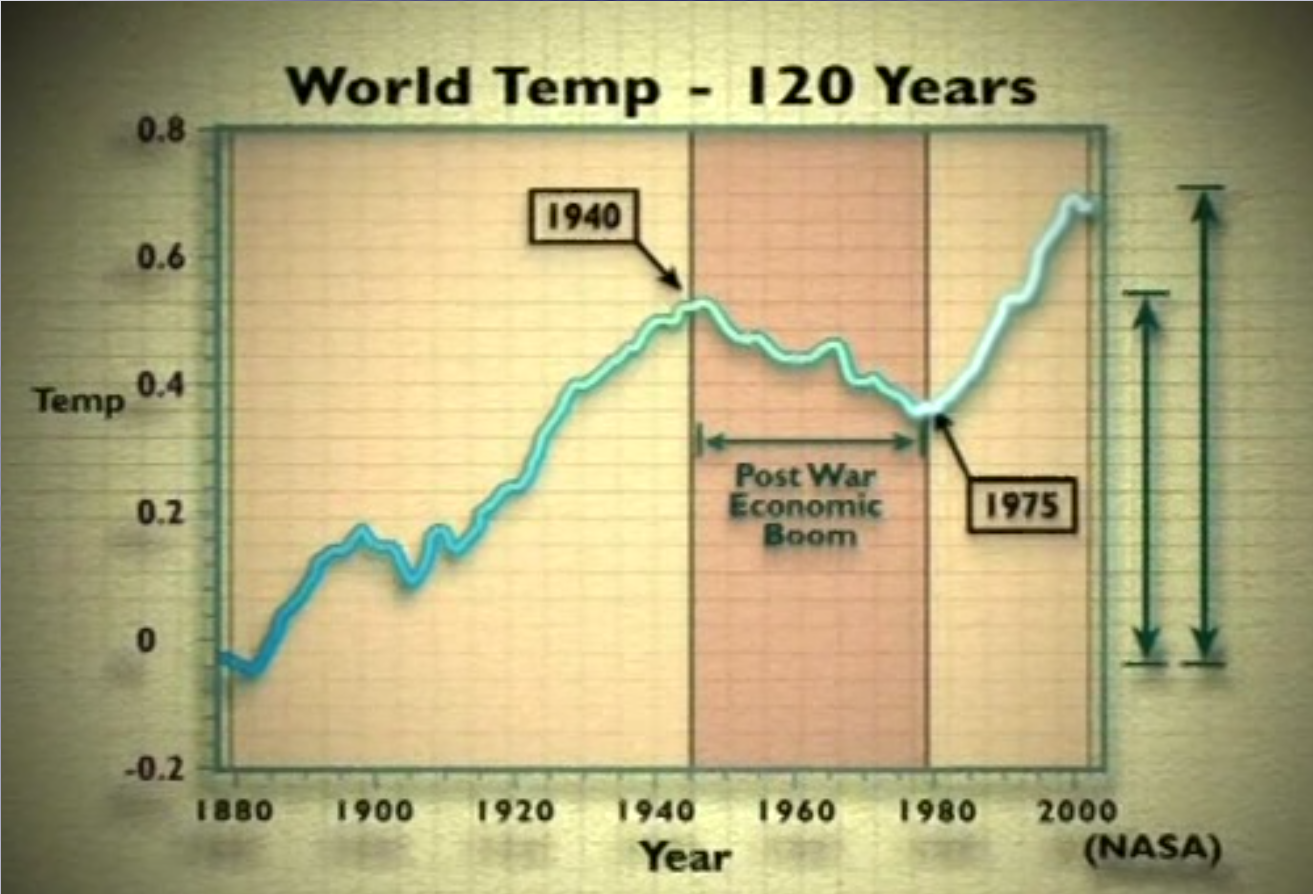
\includegraphics[scale=0.25]{fake_graph.ps}
        \caption{Global Temperature Anomaly as used by the film}
    \end{figure}
           
	- Film shows the graph\\
	- What was/is the post economic boom\\
	- How has the film interpreted the graph/data\\
	- What is the correct way of interpreting the data\\
\subsection{Global Warming is Politics}	
	- Film claims the global warming industry is political\\
	- IPCC misrepresenting scientists\\
	- Can't substantiate the claims made by the film\\
\subsection{Temperature Leads $CO_2$}
	- Film claims that T leads CO2, not the other way around\\
	- Shows famous graph\\
	- How the film interprets the data\\
	- The correct way of interpreting the graph\\
	- Scientist explanation of graph\\
\subsection{The Insignificance of $CO_2$}
	- Film claims CO2 is not major factor in greenhouse gases\\
	- Ocean is much more significant\\
	- Sun (and sun spots) actually changes the temperature\\
	- Environment needs equilibrium\\
	- Simply wrong \\
\section{Solution Presented}
	- Film says funding for global warming research should be ceased\\
	- Also that people should stop caring and doing things to stop it\\
	- Simply wrong, based on the facts. The solution doesn't stand up\\
	- Best course of action is to keep researching in the global warming field and to work together to create a cleaner society.\\
\section{Conclusion}
	- The film fails to provide concrete evidence to support their claims and solutions\\
	- The science seems to have been altered to provide seemingly convincing evidence to those not versed in the global warming field \\
	- A piece of propaganda \\
\section{References}
235

\end{document}